\documentclass[tikz,border=5pt]{standalone}
\usepackage[T1]{fontenc}
\usepackage{lmodern,amsmath,amssymb}
\usetikzlibrary{arrows.meta,calc,positioning,fit,backgrounds,shapes.geometric,matrix,decorations.pathreplacing,patterns}
\definecolor{ink}{gray}{0.08}
\definecolor{wash}{gray}{0.965}
\definecolor{soft}{gray}{0.45}
\tikzset{box/.style={draw=ink,line width=.65pt,fill=white,align=center,inner sep=4pt,outer sep=0pt,font=\small},flow/.style={draw=ink,line width=.65pt,-{Latex[length=1.8mm,width=1.3mm]},rounded corners=2pt},annotation/.style={font=\scriptsize,text=soft,align=center},groupbox/.style={draw=soft,dashed,line width=.45pt,fill=wash}}
\begin{document}
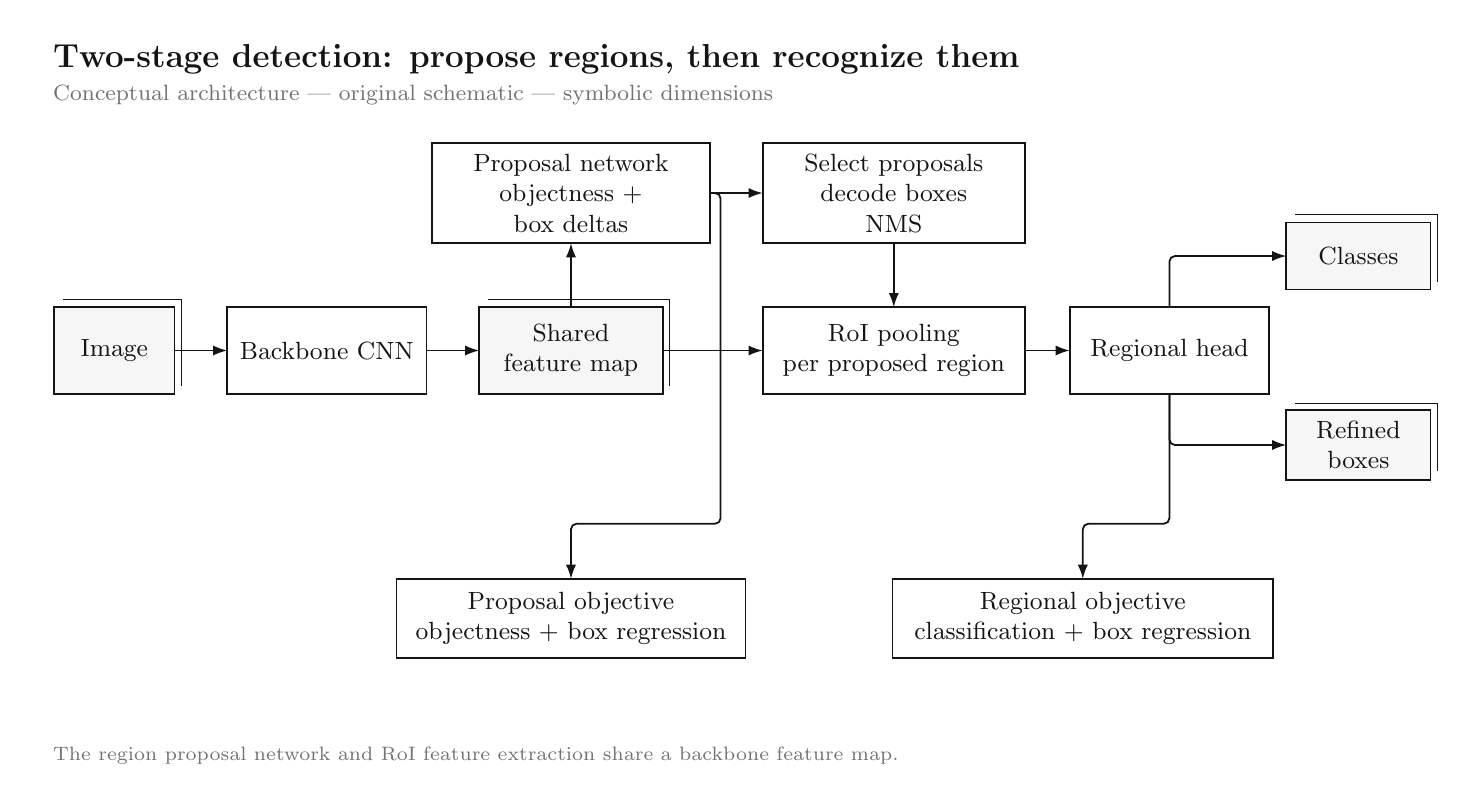
\begin{tikzpicture}[x=1cm,y=-1cm,font=\rmfamily,text=ink]

\path[use as bounding box] (0,0) rectangle (18,9.5);
\node[anchor=west,font=\large\bfseries] at (.2,.4) {Two-stage detection: propose regions, then recognize them};
\node[anchor=west,font=\footnotesize,text=soft] at (.2,.85) {Conceptual architecture | original schematic | symbolic dimensions};
\begin{pgfonlayer}{background}
\end{pgfonlayer}
\node[box,fill=wash,minimum width=1.5cm,minimum height=1.1cm,text width=1.25cm] (x) at (1.1,4.1) {Image};
\draw[ink,line width=.4pt] (0.45000000000000007,3.4499999999999997) -- (1.9500000000000002,3.4499999999999997) -- (1.9500000000000002,4.55);
\node[box,minimum width=2.5cm,minimum height=1.1cm,text width=2.25cm] (back) at (3.8,4.1) {Backbone CNN};
\node[box,fill=wash,minimum width=2.3cm,minimum height=1.1cm,text width=2.05cm] (feat) at (6.9,4.1) {Shared\\feature map};
\draw[ink,line width=.4pt] (5.85,3.4499999999999997) -- (8.15,3.4499999999999997) -- (8.15,4.55);
\node[box,minimum width=3.5cm,minimum height=1.25cm,text width=3.25cm] (rpn) at (6.9,2.1) {Proposal network\\objectness +\\box deltas};
\node[box,minimum width=3.3cm,minimum height=1.25cm,text width=3.05cm] (prop) at (11.0,2.1) {Select proposals\\decode boxes\\NMS};
\node[box,minimum width=3.3cm,minimum height=1.1cm,text width=3.05cm] (roi) at (11.0,4.1) {RoI pooling\\per proposed region};
\node[box,minimum width=2.5cm,minimum height=1.1cm,text width=2.25cm] (head) at (14.5,4.1) {Regional head};
\node[box,fill=wash,minimum width=1.8cm,minimum height=0.85cm,text width=1.55cm] (cls) at (16.9,2.9) {Classes};
\draw[ink,line width=.4pt] (16.099999999999998,2.375) -- (17.9,2.375) -- (17.9,3.2249999999999996);
\node[box,fill=wash,minimum width=1.8cm,minimum height=0.85cm,text width=1.55cm] (box) at (16.9,5.3) {Refined boxes};
\draw[ink,line width=.4pt] (16.099999999999998,4.775) -- (17.9,4.775) -- (17.9,5.625);
\node[box,minimum width=4.4cm,minimum height=1.0cm,text width=4.15cm] (loss1) at (6.9,7.5) {Proposal objective\\objectness + box regression};
\node[box,minimum width=4.8cm,minimum height=1.0cm,text width=4.55cm] (loss2) at (13.4,7.5) {Regional objective\\classification + box regression};
\begin{pgfonlayer}{background}
\draw[flow] (x.east) -- (back.west);
\draw[flow] (back.east) -- (feat.west);
\draw[flow] (feat.east) -- (roi.west);
\draw[flow] (roi.east) -- (head.west);
\draw[flow] (feat.north) -- (rpn.south);
\draw[flow] (rpn.east) -- (prop.west);
\draw[flow] (prop.south) -- (roi.north);
\draw[flow] (head.north) -- (14.5,2.9) -- (cls.west);
\draw[flow] (head.south) -- (14.5,5.3) -- (box.west);
\draw[flow] (rpn.east) -- (8.8,2.1) -- (8.8,6.3) -- (6.9,6.3) -- (loss1.north);
\draw[flow] (head.south) -- (14.5,6.3) -- (13.4,6.3) -- (loss2.north);
\end{pgfonlayer}
\node[anchor=west,align=left,font=\scriptsize,text=soft,text width=17.6cm] at (.2,9.25) {The region proposal network and RoI feature extraction share a backbone feature map.};
\end{tikzpicture}
\end{document}
